\chapter{Background}
\label{chapter:background}
This chapter provides the basics essential for the thesis.
Sect.~\ref{section:2_1_ontologies} explains ontologies and ontology languages.
Sect.~\ref{section:2_2_ontology_engineering} reviews the state-of-the-art on ontology engineering.
The last two sections explain the domain of interest of PEO.
Specifically, Sect.~\ref{section:2_3_llms} describes LLMs, while Sect.~\ref{section:2_4_prompt_engineering} surveys the state-of-the-art in prompt engineering.

\section{Ontologies}
\label{section:2_1_ontologies}
\subsection{Definition}
In AI, an ontology is a formal explicit description of a domain of interest for a certain purpose.
The main components of ontologies are classes that represent concepts, and relationships among them, e.g., class hierarchies, class disjointness and class unions.
Additionally, each class can be associated with attributes (roles) and restriction rules on the attributes (role restrictions).
Just as in object-oriented programming, classes are instantiated to create instances (individuals) \cite{protege_ontology}.

\begin{figure}[H]
    \centering
    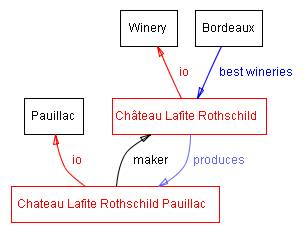
\includegraphics[width=0.5\linewidth]{Figures/fig_0.jpg}
    \caption{Example of a simple ontology in wine domain}
    \label{fig:wine_ontology}
\end{figure}
Fig.~\ref{fig:wine_ontology} depicts an example of an ontology in the wine domain; it represents wines, regions, producers.

% \subsection{Classification of ontologies}
\subsection{Classification}
In this section, we classify ontologies along multiple dimensions \cite{canfora2004ontologie}.
Firstly, ontologies can be classified according to the level of generality of the domain of discourse; specifically, from the most general to the most specific domains, as follows:
\begin{itemize}
    \item \textbf{High-level ontologies} describe very general concepts or common-sense knowledge such as space, time, objects, and actions. E.g., DOLCE ontology \cite{borgo2022dolce}.
    \item \textbf{Domain ontologies} describe the vocabulary, theories, and fundamental principles that govern a specific domain. E.g., tourism ontology \cite{tourismOntology2013}.
    \item \textbf{Task ontologies:} describe the vocabulary related to a specific task or activity, providing a specialization of the terms introduced in the high-level ontology. E.g., planning ontology \cite{taskOntologyPlanning}.
    \item \textbf{Application ontologies} describe concepts related to a specific domain or task and are often derived through a specialization of domain ontologies and task ontologies. E.g., OntoWeb \cite{ontoweb2002}.
\end{itemize}

Ontologies can differ in the level of formalism adopted. Therefore, they can be classified also as follows:
\begin{itemize}
    \item \textbf{Highly informal ontologies} are expressed in natural language, thus potentially leading to ambiguous definitions given the inherent ambiguity of natural language.
    \item \textbf{Semi-informal ontologies} are expressed in a rigid and structured form of natural language, improving clarity and reducing ambiguities.
    \item \textbf{Semi-formal ontologies} are expressed through formally defined artificial languages.
    \item \textbf{Strictly formal ontologies} are expressed with languages based on formal semantics.
\end{itemize}

A further classification can be made based on the expressiveness that the ontology aims to convey:
\begin{itemize}
    \item \textbf{Controlled vocabularies} are finite lists of terms representing the simplest possible notion of an ontology. A typical example is a catalogue that provides only terms with an unambiguous interpretation.
    \item \textbf{Glossaries} are lists of terms along their meanings expressed through natural language statements. Being primarily created for human use, they often consist of ambiguous statements that cannot be used by automated agents.
    \item \textbf{Thesauri} add semantics to glossaries by defining the relationships between terms (such as synonymy relations). Typically, they do not provide an explicit hierarchical structure, although this can be inferred from the specification of the terms.
    \item \textbf{Informal Is-A hierarchies} are ontologies in which generalization and specialization are achieved even though there is no strict "sub-class" hierarchy. They include various ontologies available on the Web.
    \item \textbf{Formal Is-A hierarchies} are ontologies in which concepts are organized according to a strict subclass hierarchy.
    \item \textbf{Frames} are ontologies in which concepts are described in terms of their characteristic properties. Inheritance relationships allow properties specified for general concepts to be inherited by more specific ones.
   \item \textbf{Logic} based ontologies represent knowledge in a formal structured manner, enabling reasoning and inference, e.g., classification and consistency check.
\end{itemize}

%  SG: parto con la definizione di ontology languages, parlo di abox e tbox e proseguo con rdf, owl, sparql e swrl
\subsection{Ontology Languages}
Ontology languages are formal languages are formal languages designed to define and represent ontologies, which describe the structure of knowledge in a specific domain.\cite{ontolang_wiki}
Knowledge in an ontology is divided into two components:
\begin{itemize}
    \item \textbf{TBox (Terminological Box):} defines the conceptual structure, including classes and properties, along with axioms that describe their relationships and constraints.

    \item \textbf{ABox (Assertional Box):} contains assertions about specific instances, describing which individuals belong to particular classes and how they relate to each other.
\end{itemize}
RDF (Resource Description Framework) is a framework used to describe graph data by using triples. Triples are used to define the ABox of an ontology, each triple has three components: 
$$
\langle subject, predicate, object\rangle
$$
The triple states that there is a relationship of type $predicate$ from the entity $subject$ to the entity $object$. Each triple component can be identified using a URI (Uniform Resource Identifier). The $object$ can be a literal or an URI while $subject$ and $predicate$ must be a URI.
For example, the triple:
\begin{lstlisting}
    <http://example.org/person/Alice> <http://example.org/knows> <http://example.org/person/Bob>.
\end{lstlisting}
it states that the resource identified by <http://example.org/person/Alice> knows (<http://example.org/knows>) a resource identified by <http://example.org/person/Bob>.
\begin{figure}[H]
    \centering
    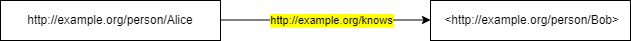
\includegraphics[width=0.9\linewidth]{Figures/fig_86.png}
    \caption{Relation between two individuals}
    \label{fig:86}
\end{figure}
Fig. \ref{fig:86} represents the RDF triple described before.

A more complex example is the following:
\begin{lstlisting}
    <http://example.org/person/Alice> <http://example.org/name> "Alice".

    <http://example.org/person/Bob> <http://example.org/name> "Bob".

    <http://example.org/person/Matt> <http://example.org/name> "Matt".

    <http://example.org/person/Alice> <http://example.org/knows> <http://example.org/person/Bob>.

    <http://example.org/person/Matt> <http://example.org/knows> <http://example.org/person/Alice>.
\end{lstlisting}
This examples involves three individuals: Alice (<http://example.org/person/Alice>), Bob (<http://example.org/person/Bob>) and Matt (<http://example.org/person/Matt>).
Each one has a name, associated with the relation <http://example.org/name> connecting the corresponding literal. Alice knows Bob, this is expressed by the triple: <http://example.org/person/Alice> <http://example.org/knows> <http://example.org/person/Bob>. Matt knows Alice, this is expressed by the triple <http://example.org/person/Matt> <http://example.org/knows> <http://example.org/person/Alice>.


\begin{figure}[H]
    \centering
    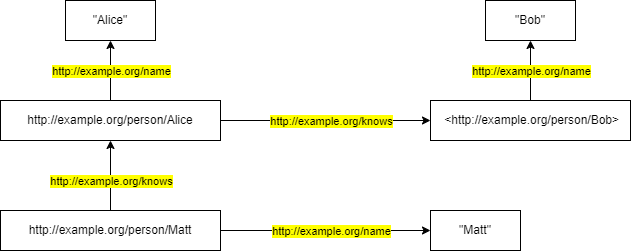
\includegraphics[width=0.9\linewidth]{Figures/fig_85.png}
    \caption{Relation between individual and name}
    \label{fig:85}
\end{figure}
Fig. \ref{fig:85} represents concepts described as an oriented labelled graph edge.

OWL is a family of knowledge representation languages for ontologies, the latest version OWL2, born in 2009, is used to build ontologies representing classes, properties, individuals, and data values that are stored as Semantic Web documents \cite{owl2}. 
OWL languages are based on DLs: a family of logic formalism derived from first order logics. 
In detail, OWL 2 is based on $SROIQ$ \cite{sroiq}. 
$SROIQ$ is a more expressive extension of previous DLs ($SHOIN$). 
$SROIQ$ introduced new features: inverse properties, cardinality restrictions, property chains and transitivity.
The main reason for choosing OWL2 is its capacity to support automatic reasoning, inferring new knowledge starting from what is represented in the ontology.
Reasoning is important to verify the consistency of the ontology, determine subsumption relations between concepts, check whether an individual belongs to a certain class and retrieve informations.
For instance, suppose we have an ontology that defines the concept of "Animal" and its subclasses, such as "Mammal" and "Bird". If we also define that "Cat" is a subclass of "Mammal", and we have an individual "Whiskers" that belongs to the "Cat" class, a reasoner can automatically infer that "Whiskers" is also a "Mammal" and an "Animal", even if these relationships were not explicitly declared.

One important aspect is the adoption of the \textit{Open World Assumption} (OWA), which implies that the absence of information does not imply its falsehood so if data are not declared we do not have informations to establish its truth.
This is useful in the semantic web where the knowledge is distributed across different sources and it is impossible to have access to all possible informations.

SPARQL is a semantic query language that allows to retrieve and manipulate data stored in RDF format.
It is based on triple patterns, i.e., statements consisting of a subject, predicate, and object, which resemble RDF triples. These triples are used to define queries that match specific data in RDF.
An example of SPARQL query is the following:
\begin{lstlisting}
PREFIX foaf:   <http://xmlns.com/foaf/0.1/>
SELECT ?name ?mbox
WHERE
  { ?x foaf:name ?name .
    ?x foaf:mbox ?mbox 
}    
\end{lstlisting}
This SPARQL query selects and returns the names (\texttt{?name}) and email addresses (\texttt{?mbox}) of entities (\texttt{?x}) that have a \texttt{foaf:name} and \texttt{foaf:mbox} property defined in the FOAF vocabulary. 

SWRL (Semantic Web Rule Language) is a language for semantic web that can be used to express logic rules, combining OWL DL with a subset of Datalog. Rules are of the form of an implication between an antecedent (body) and a consequent (head). The intended meaning can be read as: whenever the conditions specified in the antecedent hold, then the conditions specified in the consequent must also hold \cite{swrl_wiki}. An example of SWRL rule is the following:
\begin{lstlisting}
hasParent(?x1,?x2) ∧ hasBrother(?x2,?x3) -> hasUncle(?x1,?x3)
\end{lstlisting}
This SWRL rule states that if $?x1$ has a parent $?x2$, and $?x2$ has a brother $?x3$, then $?x3$ is the uncle of $?x1$. It infers family relationships in an ontology, allowing automatic reasoning about uncles based on parents and siblings.
SWRL extends OWL enabling advanced inferences but a drawback is that it can be computationally expensive and rules are not executable in all reasoners.

\subsection{Ontology repositories}
Ontology repositories facilitate the discovery of ontologies and thus their reuse, main repositories are:
\begin{itemize}
    \item W3.org \footnote{https://www.w3.org/wiki/Lists\_of\_ontologies}: a curated list of ontologies covering various domains, maintained by W3C.

    \item DBpedia \footnote{https://archivo.dbpedia.org/list}: a repository of linked data ontologies extracted from Wikipedia, enabling semantic web applications.

    \item AgroPortal \footnote{https://agroportal.lirmm.fr/ontologies?search=o}: a platform hosting agricultural and food-related ontologies for data interoperability.

    \item BioPortal \footnote{https://bioportal.bioontology.org/ontologies}: a repository of biomedical ontologies providing standardized vocabularies for health and life sciences.

    \item LOV (Linked Open Vocabularies) \footnote{https://lov.linkeddata.es/dataset/lov/}: a repository of linked data vocabularies, facilitating ontology reuse and interoperability.


    \item OntoHub \footnote{https://github.com/ontohub/ontohub}: a web-based repository for distributed ontologies, models and specifications.
\end{itemize}
Any user can contribute to these repository by submitting a new ontology or commenting and suggesting improvements to existing ontologies.



\section{Ontology Engineering}
\label{section:2_2_ontology_engineering}
% R. Richiesta modifica. Controllare la consistenza dello stile dell'espressione ontology engineering. Se ti fa comodo puoi anche definire un acronimo (OE per esempio) e usare sempre quello.

\textbf{Ontology Engineering} is the discipline that focuses on the design, development, and management of ontologies. It involves various activities such as ontology specification, knowledge acquisition, conceptualization, formalization, implementation, evaluation, maintenance, and documentation. The goal is to create structured, machine-readable knowledge representations that facilitate interoperability, reasoning, and knowledge sharing. This process relies on formal languages like OWL and RDF and employs tools such as Protégé.\cite{falquet2011introduction}
In this section, we describe the main state-of-art techniques and methodologies in ontology engineering. Finally we discuss some ontology design patterns that can be reused in the ontology design.
\subsection{Requirements Definition and Conceptualization}
The definition of requirements and the subsequent conceptualization are two fundamental tasks in ontology engineering.
They aim at establishing the objectives and scope of the ontology, and the constructs within it, respectively.
To define the scope and the requirements that the ontology should be able to address, \textbf{Competency Questions} (CQs) stand for the state-of-the-art approach.
They are questions written in natural language that the ontology should be able to answer \cite{malheiros2013method}.

For instance, in the development of an ontology for noise pollution monitoring \cite{espinoza2020using}, the following CQs have been defined:
\begin{table}[H]
    \centering
    \begin{tabular}{|>{\raggedright\arraybackslash}p{1cm}|>{\raggedright\arraybackslash}p{6cm}|>{\raggedright\arraybackslash}p{6cm}|}
        \hline
        \textbf{Id} & \textbf{Competency question} & \textbf{Answer} \\ \hline
        \textbf{CQ1} & Which is the measured noise level in a specific moment and location? & The detected noise level during April in location with coordinates 40.42, – 3.69, 648 is 67.4 dB. \\ \hline
        \textbf{CQ2} & Which is the location of a specific measurement station? & The location of the measurement station “Paseo de Recoletos” is 40.42, – 3.69, 648 (Longitude, Latitude, Altitude) \\ \hline
        \textbf{CQ3} & In which day interval the noise level has been detected? & The noise level Ld has been detected in the time interval between 07:00 to 19:00. \\ \hline
        \textbf{CQ4} & Which was the last calibration sensor date? & The datetime, for example, 2017-04-21T14:00:00+01:00 \\ \hline
    \end{tabular}
    \caption{Competency Questions noise pollution ontology}
\end{table}
Each CQ must correspond to a natural language answer that "simulates" the response provided by the ontology.
CQs are translated into SPARQL queries in order to be executed on the ontology.
Once defined, CQs can be used for evaluating an ontology.

The conceptualization (or design) of the ontology aims at defining the classes, the relationships among them, and the individuals.
There are three approaches to conceptualization:
\begin{enumerate}
    \item \textbf{Top-down} development process starts with the definition of the most general concepts in the domain and subsequent specialization of the concepts.
    \item \textbf{Bottom-up} development process starts with the definition of the most specific classes, the leaves of the hierarchy, with subsequent grouping of these classes into more general concepts.
    \item \textbf{Hybrid} development process is a combination of the top-down and bottom-up approaches: we define the most salient concepts first and then generalize and specialize them appropriately.
\end{enumerate}

\subsection{Ontology Engineering Methodologies}
\textit{METHONTOLOGY} \cite{fernandez1997ontological} proposes a structured method consisting of six steps:  
Firstly, the specification phase aims at producing the ontology specification document, outlining the main requirements and the scope of the ontology.
It can be informal, semi-formal, or formal, and is written either in natural language or using CQs.
Next, the \textsf{knowledge acquisition} phase involves gathering all relevant knowledge related to the domain. 
It can be performed based on various techniques, such as text analysis, brainstorming, interviews, and reviewing existing similar ontologies.

The \textsf{conceptualization} phase follows, where the acquired knowledge is organized into a conceptual model.
During the \textsf{integration} phase, the methodology encourages reusing and integrating existing ontologies rather than developing new ones from scratch. 
This step is crucial for ensuring consistency and coherence, as it involves checking libraries of ontologies to find definitions of terms that match the semantics identified in the conceptualization phase.
The \textsf{implementation} phase is where the actual construction of the ontology takes place.
Finally, the \textsf{evaluation} phase ensures the quality and correctness of the ontology.
This step involves both verification, to confirm that the ontology is semantically sound, by using a reasoner, and validation.

The methodology has the following advantages: 
\begin{itemize}
    \item It proposes the use of an evolutionary prototype life cycle, which allows definitions to be modified, added or removed at any time.

    \item It encourages the reuse of already existing ontologies, which can speed up development and ensure consistency with other projects. 
\end{itemize}

However, it also has disadvantages:
\begin{itemize}
    \item The methodology is very detailed and rigorous, which can be time and resource consuming, especially for smaller projects, it may be excessive compared to the needs of the project.

    \item The methodology can be complex to master for those without experience in ontology development, as it requires familiarity with several specific techniques and tools.

    \item The methodology has been developed in 1997, making it outdated by today standards. Since its creation, there have been significant advancements in both ontology engineering and related technologies, such as the Semantic Web, Linked Data, and agile methodologies.

    \item The methodology was created before the widespread adoption of agile development practices, which are now a common approach in software and ontology engineering. This makes it less flexible for fast-paced, iterative development environments.
\end{itemize}

Another proposed methodology is the \textit{NeOn} methodology \cite{neon1,neon2}, which provides guidance for all key aspects of the ontology engineering process.
The concepts underlying this methodology are: scenarios, collaborative ontology development, reuse of ontological and non-ontological resources and evolution of networked ontologies. 

The ontology engineering is based on nine scenarios:
\begin{itemize}
    \item \textbf{Scenario 1: from specification to implementation} The ontology network is developed from scratch, engineers should specify ontology requirements and search for potential resources to be reused. 

    \item \textbf{Scenario 2: reusing ontological resources} Engineers reuse ontological resources, ontology modules and ontology statements to build ontology networks. 

    \item \textbf{Scenario 3: reusing and re-engineering ontological resources} Ontology engineers reuse and re-engineer ontological resources

    \item \textbf{Scenario 4: reusing and merging ontological resources} This scenario arises when several ontological resources in the same domain are selected for reuse, and engineers wish to create a new ontological resource with the selected resources

    \item \textbf{Scenario 5: reusing, merging and re-engineering ontological resources} Ontology engineers reuse, merge, and re-engineer ontological resources. 
    This scenario is similar to Scenario 4, but here engineers decide to re-engineer the set of merged resources

    \item  \textbf{Scenario 6: reusing ontology design patterns} Ontology engineers access repositories to reuse design patterns

    \item \textbf{Scenario 7: ontology engineers access repositories to reuse design patterns} Ontology engineers restructure (e.g., modularize, prune, extend, and/or specialize) ontological resources to be  integrated in the ontology network. 

    \item \textbf{Scenario 8: localizing ontological resources} Ontology engineers adapt an ontology to other languages and culture communities, thus obtaining a multilingual ontology.

\end{itemize}
The scenarios presented are not a rigid workflow, they are more like a variety of pathways for developing ontologies and they cover commonly occurring situations, for example, when available ontologies need to be re-engineered, aligned, modularized, localized to support different languages and cultures, and integrated with ontology design patterns and non-ontological resources, such as folksonomies or thesauri\cite{suarez2011neon}.

The \href{http://neon-project.org/nw/Welcome_to_the_NeOn_Project.html}{Neon project} offers to engineers a tool called \href{http://neon-toolkit.org/wiki/Main_Page.html}{NeOn toolkit}: an open-source multi-platform ontology editor which supports OWL2 and features basic editing and visualization functionalities \cite{erdmann2011overview}.

\begin{figure}[H]
    \centering
    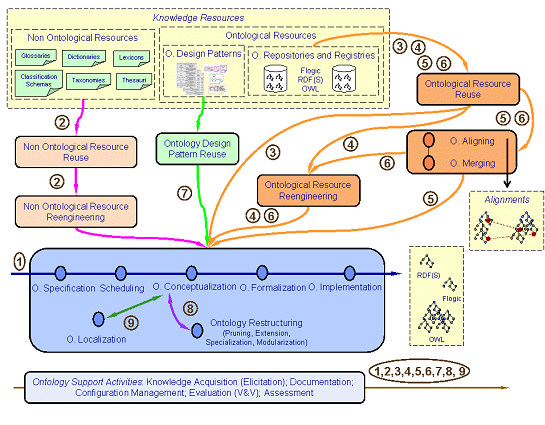
\includegraphics[width=0.5\linewidth]{Figures/fig_2.png}
    \caption{\textit{NeOn} methodology scenarios}
    \label{fig:2}
\end{figure}
Fig.~\ref{fig:2} represents the different scenarios in the NeOn methodology.
The \textit{NeOn} methodology has the following advantages:
\begin{itemize}
    \item It identifies nine different scenarios for building ontology networks, which can be combined depending on the project’s needs, this contrasts with more rigid methodologies like \textit{METHONTOLOGY}.

    \item It supports the reuse and re-engineering of both ontological and non-ontological resources, which can save time and effort by leveraging existing knowledge bases, reducing the need to build everything from scratch.

    \item By basing its structure on real use cases and generalizing from them, the \textit{NeOn} methodology covers practical needs encountered in ontology development projects.
\end{itemize}
However, \textit{NeOn} has the following disadvantages:
\begin{itemize}
    \item The flexibility and comprehensive nature of the methodology can make it more complex to apply, especially for teams without significant prior experience in ontology development. 

    \item Although \textit{NeOn} is designed for building large-scale networks, the actual process of merging and aligning different ontologies can be challenging, especially when ontologies come from diverse sources with differing structures and standards.

    \item The methodology is meant to be technology-independent, in practice, it may require specific tools to implement the processes effectively, and these tools might not always be accessible or easy to use for all teams.
\end{itemize}

While the \textit{NeOn} methodology is scenario-based, the \textit{eXtreme Design} (XD) methodology \cite{presutti2009extreme} is based on a sequence of tasks inspired by the principles of agile development in software engineering.
XD involves the stakeholders in order to gather complete requirements without making incorrect assumptions.
This interaction is useful for defining CQs and user stories that detail the use of the ontology, supported by contextual statements that make implicit knowledge explicit.
The principles of XD not only focus on the customer, but also provide clear guidelines to engineers regarding the design and organization of work.
In particular, the design must be modular and task-oriented, focusing on the specifications defined in the CQs.
The CQs are used in the development of unit tests during the testing phase, verifying the compliance of the ontology with the customer stories.
Tests are generally conducted using SPARQL queries that encode the CQs.
Throughout the development phase, the engineers are organized according to the \textit{pair design}, where the design team is divided into pairs that must collaborate, by sharing knowledge.
Based on the illustrated principles, XD defines the following tasks: 
% \begin{enumerate}
\begin{itemize}
    \item \textbf{Task 1. Get into the project context:} the development process begins by aligning the engineers and domain experts, who may have different backgrounds and terminologies. The goal is twofold: to familiarize the customer with the project's methods and tools, and to provide the engineers with an understanding of the problem, scope, and initial terminology as well as establishing a collaborative environment for sharing documentation and discussing modelling issues.

    \item \textbf{Task 2. Collect requirement stories:} the customer writes stories starting from real scenarios in order to provide examples of the typical facts that should be stored in the ontology.

    \item \textbf{Task 3. Select a story that has not been treated yet:} each pair of engineers selects a story to focus on for the next iteration for releasing an ontology module. They create a new wiki page with the story's title and content based on the information from the card.

    \item \textbf{Task 4. Transform the story into CQs:} create a sequence of CQs, this task involves customer for having feedback/clarifications.

    \item \textbf{Task 5. Match the CQ to use cases:} identify candidate Content Patterns (CPs) (a specific type of ontology design patterns, see Sect.~\ref{subsection:2_2_ontology_design_patterns}) based on the CQs that express part of the ontology to be modelled. Matching can be done with tool support, such as keyword-based searching, or manually by engineers familiar with available CPs.

    \item \textbf{Task 6. Select the CPs to reuse:} select which of those patterns should be used for solving the modelling problem.

    \item \textbf{Task 7. Reuse and integrate selected CPs:} apply typical operations for CPs i.e. import, specialization, and composition. 

    \item \textbf{Task 8. Test and fix:} validate the module by ensuring it aligns with the CQs just modelled. This process involves several steps: first, the CQ is transformed into a unit test, such as a SPARQL query, then, the module is populated with sample data based on the story, and the test is run. If the result isn't as expected, the module is revised and the test is rerun until it passes and once all tests linked to the story have been successfully completed, the engineers can move on to the next task. If any CQ remains unaddressed, they return to an earlier task to make adjustments.

    \item \textbf{Task 9. Release module:} release an ontology module having an URI shared with the whole team and on web repositories.

    \item \textbf{Task 10. Integrate, test and fix:} integrate the module with the other modules that constitute the ontology.
\end{itemize}

Once the eleven tasks have been completed, the release of the new version of the ontology takes place.
The XD methodology has the following advantages:
\begin{itemize}
    \item The methodology supports collaboration and modular ontology development, allowing teams to work on different parts of the ontology in parallel, which is especially useful for large and distributed projects.

    \item It employs a test-driven approach, where CQs and contextual statements serve as the basis for unit testing the ontology, ensuring that each component meets its intended purpose before moving forward.

    \item The methodology emphasizes constant interaction with domain experts and stakeholders to ensure that the ontology meets the intended use and requirements. This minimizes assumptions and ensures that implicit knowledge is captured.
\end{itemize}
However, there are also disadvantages:
\begin{itemize}
    \item The methodology's iterative, test-driven nature may be overkill for smaller ontology projects, where a simpler, more direct approach could be more efficient.

    \item Effective use of XD relies on the availability of supporting tools, such as the \textit{NeOn} Toolkit and its XD plugin. While these tools are valuable, they may limit accessibility if they are not well-maintained or widely available.
\end{itemize}

The \textit{Linked Open Terms} (LOT) methodology \cite{poveda2022lot} is a lightweight industrial-oriented methodology for ontology engineering.
The methodology is compatible with software engineering methodologies; indeed, it is inspired by the agile methodology.
\begin{figure}[H]
    \centering
    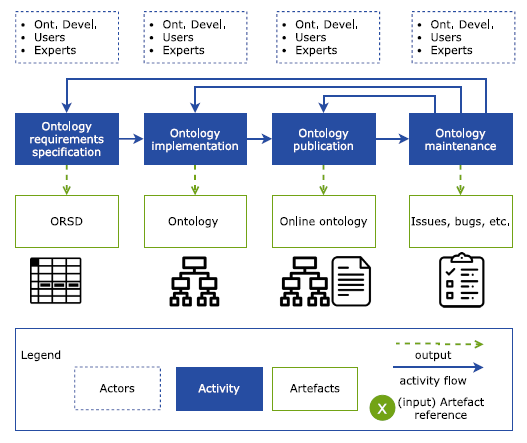
\includegraphics[width=0.7\linewidth]{Figures/fig_3.png}
    \caption{LOT methodology base workflow}
    \label{fig:lot-workflow}
\end{figure}

Fig.~\ref{fig:lot-workflow} describes the ontology development lifecycle with four stages: requirements specification, implementation, publication, and maintenance, involving collaboration between ontologists, developers, users, and experts.
Each stage outputs artefacts (e.g., ORSD, ontology, online ontology) that flow into subsequent phases for iterative refinement and usage.

This phase aims at defining the domain of interest, the goal of the ontology and the implementation language.
In detail, there are seven steps as described below.
Initially, use case specifications are created in collaboration with domain experts, users, and ontology engineers.
These use cases describe scenarios in which the ontology will be utilized and are expressed in natural language.
Next, data exchange identification is carried out, where the necessary documentation and resources related to the domain are gathered and compiled into a set of documents.
The purpose and the scope of the ontology are then identified with input from users and domain experts.
The purpose clarifies the reason for creating the ontology, while the scope defines the aspects of the domain that will be represented.

Subsequently, a set of functional ontological requirements is proposed, often in the form of CQs or natural language statements.
These requirements outline what the ontology should be able to answer and represent. 
Ontology experts then review these functional requirements to ensure their correctness and completeness, addressing any ambiguities and verifying consistency with the defined purpose and scope.
Following this, the \textit{Ontology Requirements Specification Document} (ORSD) is formalized.
This document consolidates all the information, CQs, and functional requirements defined in the earlier phases, serving as a comprehensive reference for the ontology engineering. 
In some cases, an optional activity is conducted where the functional ontology requirements are further formalized into test cases, expressed in SPARQL queries.
This step helps in validating that the ontology meets the specified requirements through structured testing.

In this phase, the ontology is implemented using a formal language.
Firstly, it involves the conceptualization, which aims at defining the constructs in the ontology.
Next, the encoding phase aims at actually implementing the ontology using an implementation language; in this phase, is useful to take into account other similar ontologies that could be reused.
Once the whole ontology is completed, it can be evaluated according to different evaluation criteria.

In this phase, the ontology is published online, making it accessible and searchable by users. 
Before publishing the ontology online, it is necessary to identify the version to be released, document the ontology using human-readable HTML pages, and finally publish the ontology online according to the W3C guidelines \cite{ontology_online}.

The last step is the ontology maintenance.
In this phase, once the ontology is published online, bug detection is performed.
Moreover, the ontology can be updated according to new requirements.

Despite being introduced recently, the LOT methodology has been widely applied successfully, both in research and in the industrial field.
In the industrial and manufacturing sector, the ontology \textit{SAREF4INMA} \cite{de2020saref4inma} has been developed to describe equipment, materials, products, factories and manufacturing processes in a structured way. 
The industry is not the only sector where an ontology developed with the LOT method can be applied.
In Spain, specifically in Madrid, an ontology has been developed to represent the Bus Public Transport system \cite{ruckhaus2023applying}. 
The ontology represents information on lines, routes, journey patterns and their timetables, stODPs on each route, information on expected bus arrival times for each stop, and information on incidents that may affect the bus routes and their journeys.
Still in Spain, the LOT methodology has been successfully used in the development of a noise pollution ontology \cite{espinoza2020using}.
The ontology integrates data from Internet of Things (IoT) sensors in the city and establishes semantic relationships between them.

The LOT methodology has been used also in AI research field, the \textit{HALO ontology} \cite{nananukul2024halo} has been creating for representing hallucinations in LLMs.
The ontology represents LLMs, hallucinations, prompts and responses.
The ontology consists of two modules and was created from a dataset of 40 known prompts designed to generate hallucinations.
Each prompt was given as input to three LLMs: ChatGPT, BARD, and Claude.
\begin{figure}[H]
    \centering
    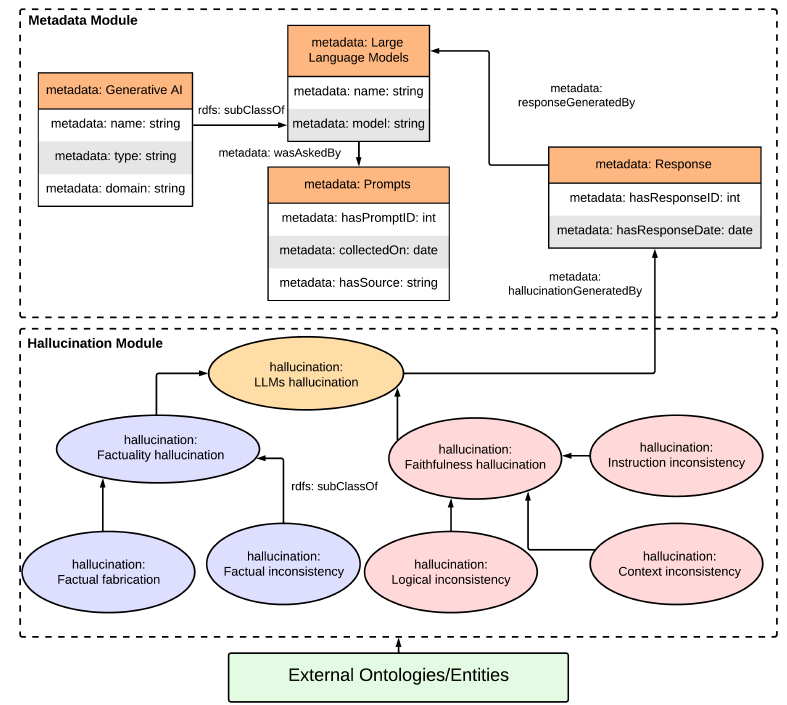
\includegraphics[width=0.7\linewidth, height=8cm]{Figures/fig_4.png}
    \caption{HALO ontology}
    \label{fig:halo}
\end{figure}
Fig. \ref{fig:halo}

The LOT methodology has the following advantages:
\begin{itemize}
    \item The LOT methodology is designed to be lightweight and agile, which allows for faster iterations and easier integration with software development practices and it is particularly well-suited for projects that need rapid, iterative development.

    \item It offers flexibility by combining various techniques (CQs, natural language statements ...) to define requirements and allows for different levels of formality depending on the project.

    \item Many open source ontologies have been developed successfully using the LOT methodology, e.g., the public transport ontology.
\end{itemize}
But, the LOT methodology has two disadvantages:
\begin{itemize}
    \item LOT encourages the reuse of existing ontologies, but this can be challenging due to the potential inconsistencies and heterogeneity of reused ontologies. However, the methodology does not fully address how to resolve these issues.

    \item The emphasis of LOT on formal validation processes (such as the use of SPARQL queries) may not be sufficient for certain complex domains or non-technical stakeholders.
\end{itemize}

\subsection{Ontology Engineering using Large Language Models}
The methodologies analysed for ontology design involve users, domain experts, and ontology engineers, but do not include the use of advanced tools based on artificial intelligence, such as LLMs. The study "From human experts to machines: An LLM supported approach to ontology and knowledge graph construction" \cite{kommineni2024human} introduces a semi-automatic pipeline for the construction of knowledge graphs. There are six phases in the proposed pipeline.
The process begins with the data collection phase, which does not involve the use of large language models (LLMs). Instead, domain experts generate a dataset and a set of publications relevant to the topic under study.
In the next phase, known as competency question (CQ) generation, ChatGPT-3.5 is utilized to create competency questions. These questions are designed to describe the data collected in the previous phase at an abstract level. Domain experts provide inputs to the LLM to generate these questions, which are then evaluated by two domain experts to ensure their relevance and accuracy. Following this, the ontology creation phase is initiated. It builds on the competency questions generated earlier. This phase involves two steps: in the first step, a prompt is created that includes a competency question, the expected output, and a set of instructions. In the second step, the LLM is provided with a basic ontology structure containing the concepts and relationships derived from the competency questions.
The CQ answering phase involves applying text processing techniques to extract answers to the competency questions. These answers are used to enrich the ontology and provide a deeper understanding of the dataset.
During the knowledge graph (KG) construction phase, the competency questions, their answers, and the ontology generated by the LLM are combined and provided as input to the LLM. The prompt for this phase focuses on extracting entities, relationships, and concepts and mapping them onto the ontology, thereby creating a comprehensive knowledge graph.
Finally, in the evaluation phase, the LLM evaluates the competency questions and the constructed knowledge graph by comparing them to a ground truth generated by human evaluators. The LLM assigns a score based on the alignment of the generated knowledge graph with the human-generated ground truth.
The presented method enabled the creation of a fairly complex ontology consisting of 45 classes, 41 relations, and 365 axioms. However, it required significant computational resources, as an 80GB NVIDIA A100 GPU machine was used. 
Another approach for ontology learning using large language models is NeOn-GPT \cite{fathallah2024neon}. Starting from the NeOn methodology, the methodology is converted to a series of prompts to ChatGPT-3.5, these prompt are created using prompt engineering techniques and they are used first to generate ontology specification and competency questions. ChatGPT-3.5 is used also to generate a conceptual model of the ontology in the form of subject-relation-object triples and to generate implementation code. Once the code is generated, there is the syntax validation using the RDFLib python library \cite{rdflib} and the consistency check in order to check logical inconsistencies. The final step is the pitfall resolution for checking circular axioms and missing disjointedness using OODPs API. The presented methodology is an evolution of the NeOn methodology, in which all tasks traditionally performed by the engineer are delegated to ChatGPT. This includes identifying requirements, writing competency questions, conceptualizing, and implementing the ontology.%\\
ChatGPT can be used not only for the creation of ontologies but also for the creation of more complex knowledge graphs, specifically Hyper-Relational Knowledge Graphs, as discussed in the study "Construction of hyper-relational knowledge graph using pre-trained large language models" \cite{datta2024construction}. Hyper-relational knowledge graphs unlike the normal knowledge graphs incorporate additional qualifiers or attribute-value pairs \cite{hyper}, in the study starting from HyperRED dataset, a dataset about different topics , the hyper relational knowledge graph is built including in prompts the data from the dataset. Prompts are generated using Chain-of-Thoughts prompt engineering technique (CoT) and in order to evaluate the result generated, BERTScore is choose as a metric. The results obtained were not satisfactory, as the other algorithm(CubeRE)for extracting hyper-relational information was not surpassed.
In general, large language models have shown promising potential  in automating and enhancing the processes of ontology and knowledge graph construction replacing the ontology engineer in different tasks.

\newpage
\subsection{Ontology Design Patterns}
\label{subsection:2_2_ontology_design_patterns}
In ontology engineering, \textit{Ontology Design Patterns} (ODPs) \cite{odps} are a powerful approach for addressing recurring problems in the design of ontologies \cite{hitzler2016ontology}.

An OP is a modelling solution for solving a recurrent ontology design problem \cite{gangemi2009ontology}.
These patterns encapsulate best practices, enabling ontology engineers to draw from proven solutions when confronted with similar challenges and enabling them to optimize time and costs during the design. 

In \cite{falbo2013ontology} there are five types of ODPs:
\begin{enumerate}
    \item \textbf{Structural ODPs}

    \item \textbf{Reasoning ODPs}

    \item \textbf{Correspondence ODPs}

    \item \textbf{Presentation ODPs}

    \item \textbf{Lexico-Syntactic ODPs}

    \item \textbf{Content ODPs}
\end{enumerate}
We describe each type in detail below.

Structural ODPs are high-level modelling solutions that address architectural and logical challenges in ontology design.
They include two main subtypes:
\begin{itemize}
    \item \textbf{Logical ODPs:} these are combinations of logical constructs that resolve expressivity issues in ontology languages. They operate independently of specific content domains and are designed to bridge gaps where a representation language lacks built-in constructs. For example, Logical ODPs help model n-ary relations in OWL, which only supports binary relations.

    \item \textbf{Architectural ODPs:} these patterns influence the overall shape and structure of an ontology. They can be internal, focusing on consistent use of Logical ODPs within an ontology or external, involving meta-level constructs like modular networks connecting multiple ontologies.
\end{itemize}

Reasoning ODPs are applications of Logical ODPs specifically designed to achieve certain reasoning outcomes.
Examples of Reasoning ODPs include classification, subsumption, inheritance, materialization, de-anonymization, and others.
When applied to an ontology, Reasoning ODPs provide insights into the state of the ontology and enable a system to determine the type of reasoning required to perform tasks such as queries, evaluations, and more.

Correspondence ODPs are a type of ODP that focuses on addressing relationships and transformations between ontologies or between ontologies and non-ontological resources.
They are divided into two main types:
\begin{itemize}
    \item \textbf{Re-engineering ODPs:} provide guidelines for transforming ontological and non-ontological models, such as database schemas or thesauri, into ontologies. 

    \item \textbf{Mapping ODPs:} These focus on creating semantic associations between elements of different ontologies without altering their structure. They help define equivalence, containment, and overlap relations as well as their negative counterparts.
\end{itemize}

Presentation ODPs focus on improving the usability and readability of ontologies from a user perspective.
They serve as best practices to enhance reusability by making ontologies easier to evaluate and select.
Key types include:
\begin{itemize}
    \item \textbf{Naming ODPs:} provide conventions for naming ontology elements (classes, properties, files, namespaces). These ensure consistency and improve human readability and understanding.

    \item \textbf{Annotation ODPs:} define annotation properties or annotation property schemas that add metadata to ontology elements, enhancing their understandability and context.
\end{itemize}
For example, a Naming OP might recommend using the base URI of the publishing organization (e.g., http://www.example.org/ontologies/) to ensure clarity and consistency.
Annotation ODPs could include descriptive metadata, such as the purpose or scope of a class.
These patterns are essential for supporting effective reuse, adaptation, and user accessibility in diverse domains.

Content Patterns (CPs) are conceptual ODPs that address domain-specific modelling issues in ontologies.
Unlike Logical ODPs, which are general and conceptualization-independent, CPs focus on solving content problems by proposing patterns for modelling domain-specific classes and properties.
CPs are reusable through specialization, extension, or composition and impact only the ontology regions addressing particular modelling problems.
Although language-independent in theory, CPs require implementation for practical reuse, often using OWL.

Lexico-Syntactic ODPs are linguistic structures or patterns composed of specific word types arranged in a particular order.
These patterns allow for generalization and enable the extraction of conclusions about the meaning they convey.
They are particularly useful for linking basic Logical and Content ODPs with natural language sentences, such as in educational or instructional contexts.

A more practical approach to ODPs is given by the \textit{Modular Ontology Design Library} (MODL) \cite{shimizu2019modl}.
MODL is a curated, well-documented, and structured collection of ODPs implemented in OWL designed to support modular ontology design.
This library promotes the FAIR (\textit{Findable}, \textit{Accessible}, \textit{Interoperable}, and \textit{Reusable}) guiding principles for scientific data management and stewardship by addressing challenges like ontology reusability and interoperability.
The library includes five categories of patterns: meta-patterns, organization of data, space-time movement, agents and roles, description, and details.
MODL offers patterns for dynamic processes, complex roles, and detailed relationships like part-whole hierarchies.
Its diversity ensures modularity and expressiveness for both general and domain-specific needs.

\section{Large Language Models}
\label{section:2_3_llms}
\subsection{Introduction and Classification}
LLMs, as seen before, are capable of supporting ontology engineering.
More broadly, this revolutionary AI technology is applied to various tasks across diverse domains, mainly because of their remarkable performance and versatility.
A LLM is a large-scale, pre-trained statistical LM based on neural networks; it is capable of natural language generation, which can be used to frame a large variety of \textit{Natural Language Processing} (NLP) tasks \cite{zhao2023survey}.
LLMs are trained on a vast amount of training data in order to predict the next word in a given sequence of words of any length, language and even including mathematical formulas and code \cite{zhao2023survey}.
LLMs are able to execute different heterogeneous tasks thanks to an underlying complex neural-network, with transformer architecture being the most advanced.
Introduced in the 2017 by the seminal paper ``\textit{Attention Is All You Need}'' \cite{vaswani2017attention}, the transformer architecture is composed by two parts:
\begin{enumerate}
    \item \textbf{Encoder:} a multilayer component where each layer consists of a multi-head self-attention mechanism and a position-wise fully connected feed-forward network.
    
    \item \textbf{Decoder:} a multi-layer component that processes the encoder's output. Each layer is based on a modified self-attention mechanism that prevents future positions from influencing past positions, ensuring autoregressive property.
\end{enumerate}
\begin{figure}[H]
    \centering
    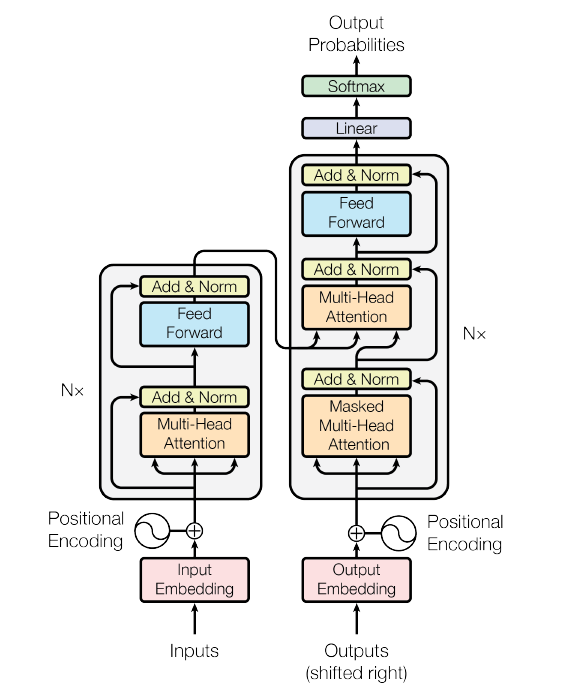
\includegraphics[width=0.5\linewidth]{Figures/fig_17.png}
    \caption{Transformer architecture}
    \label{fig:17}
\end{figure}
Fig.~\ref{fig:17} depicts the transformer architecture with with the encoder (on the left) and the decoder (on the right).
Two different variants of the transformer architecture have been adopted:
\begin{itemize}
    \item \textbf{Encoder-Decoder:} processes inputs through the encoder and passes the intermediate representation to the decoder to generate the output \cite{encoder_medium}.

    \item \textbf{Decoder-only:} does not have an encoder and it uses a decoder in order to generate tokens, each token depends on the previous sequence \cite{uniteai_decoder}.

    \item \textbf{Encoder-only:} does not have a decoder and it processes the entire sequence simultaneously generating contextualized representations for each token\cite{ewer2024entp}.
\end{itemize}

The simplicity and versatility of the decoder-only architecture allows for reaching extremely large scale (billions of parameters and hundreds of gigabytes of training data).
Such an unprecedented scale endowed LLMs with the so-called emerging abilities.
They made LLMs able to solve a large variety of tasks with remarkable performance with no need for additional re-training or fine-tuning, but simply needing to be prompted.
Indeed they are also called \textit{general purpose} LLMs or \textit{Foundation Models}.
Such emerging abilities include:
\begin{itemize}
    \item \textit{Instruction following:} the ability of an LLM to execute commands and respond coherently to user instructions.

    \item \textit{In-context learning:} the capability to learn and generalize from examples provided within the same interaction session, without updating the model’s weights.

    \item \textit{step-by-step problem solving:} the ability to break down complex problems into simpler steps, following a structured process to reach a solution.
\end{itemize}
Such abilities constitute the basis for the definition of effective prompts.
Despite being less general than GPT, also BERT and T5 are often considered \textit{Foundation Models} as they have represented crucial milestones in the development of LLMs.
Moreover, for classification (summarization) tasks, BERT (T5) can still outperform GPT and other very large decoder-only LLMs.

\subsection{General Purpose Large Language Models}
General purpose LLMs are capable of performing a wide variety of tasks.
In this section, we will analyse and discuss the following state-of-the-art general purpose LLMs:
\begin{itemize}
    \item \textbf{GPT}
    \item \textbf{BERT}
    \item \textbf{PaLM}
    \item \textbf{LLaMA}
    \item \textbf{T5}
    \item \textbf{BLOOM}
    \item \textbf{Mistral}
\end{itemize}

The \textit{Generative Pre-trained Transformer} (GPT), released by Open AI, is actually the most advanced and powerful LLM available to users.
In two months, it gained over than 100 million of users, making it the fastest-growing consumer software application in history \cite{achiam2023gpt}.
GPT is a decoder-only LLM.

Since its first version, GPT-1 released in 2018, the model has represented a step forward in AI.
GPT-1 has 117 million parameters and is trained on the BookCorpus dataset.
The model has been improved in 2019 with the next version GPT-2, which has 1.5 billions of parameters and is trained on WebText dataset with 8 millions of documents \cite{radford2019language}.
In 2020, OpenAI has released GPT-3, which has 175 billions of parameters and is trained over one trillion of documents.
The latest version of GPT is GPT-4; it is a multimodal model, i.e., it can take as input both images and text and generate a response consisting of both images and text.
Despite the continuous evolution and the billions of parameters of the model, it is still subject to issues, including hallucinations \cite{achiam2023gpt}.
In general, an hallucination is a response generated by an AI model that contains false or misleading information presented as a fact. An example of hallucination is the following:
\begin{lstlisting}
Prompt: Who won the 2024 Formula 1 constructors world championship?
Response: The Redbull team won the Formula 1 constructors world championship in 2024
\end{lstlisting}
The response is wrong because McLaren team won in 2024 the Formula 1 constructors world championship in 2024.
Another example is:
\begin{lstlisting}
Solve the equation: 3x - 11 = 5
Response: x = 4
\end{lstlisting}
The response is wrong because the correct result is $5.33$ given by $x = \frac{11+5}{3}$.

GPT is a proprietary LLM, so its parameters and training set are not publicly available.
GPT has been made available to the public as a web application called ChatGPT and represented in Fig.~\ref{fig:18}.

\begin{figure}[H]
    \centering
    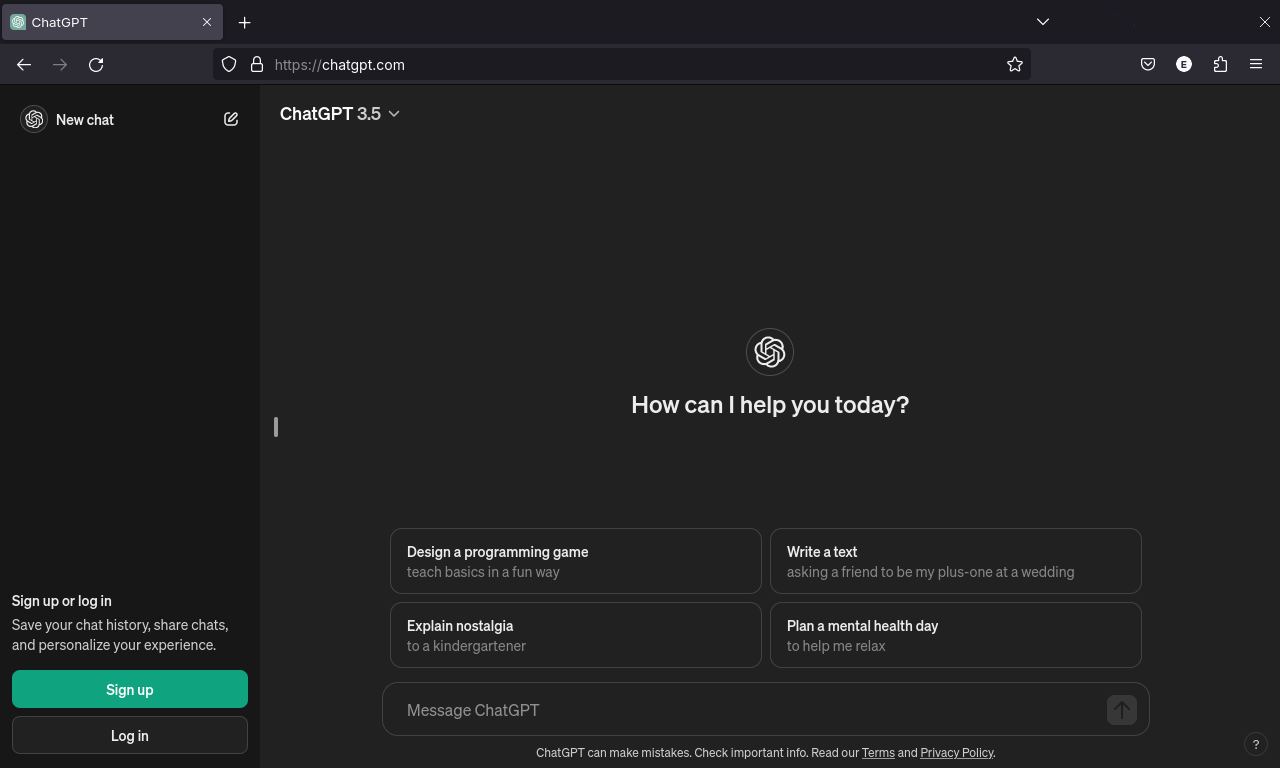
\includegraphics[width=0.9\linewidth]{Figures/fig_18.png}
    \caption{ChatGPT interface}
    \label{fig:18}
\end{figure}

\textit{Bidirectional Encoder Representations from Transformers} (BERT) was introduced by Google AI in 2018 \cite{kenton2019bert}.
BERT is a encoder-only LLM.
Compared to other models like GPT, BERT is a bidirectional model: it takes into account the context on the left and on the right of each input word.
It has 340 milions of parameters.
It is trained on the BookCorpus dataset \cite{bandy2021addressing} and on english Wikipedia. BERT is an open-source LLM.

Unlike GPT, it does not have a web interface, but the different versions of BERT are available for download on Huggingface \footnote{https://huggingface.co/docs/transformers/model\_doc/bert}.

In September 2023, Google AI released \textit{Pathways Language Model} (PaLM).
It is a decoder-only LLM.
It has 540 billions of parameters and is trained with the Pathways system that allows parallel training \cite{anil2023palm,barham2022pathways}.
PaLM is trained using a combination of English and multilingual datasets (100 languages) that include high-quality web documents, books, Wikipedia, conversations, and GitHub code in order to learn to perform complex reasoning and code generation tasks\cite{palm2_intro}.
PaLM is a proprietary model and it is available on the official website\footnote{https://cloud.google.com/vertex-ai/generative-ai/docs/language-model-overview?hl=it\#palm-api}.
PaLM serves as the starting point for an even more powerful multimodal model: Google Gemini, which will be discussed later.

\textit{Large Language Model Meta AI} (LLaMA) is a family of LLMs introduced in 2023 by another web giant: META.
LLaMA models are decoder-only LLMs.
The latest version LLaMA 3 includes over 400 billions of parameters \cite{llama3_intro}.
LLaMA models, like PaLM, are trained using different sources, specifically: EnglishCommonCrawl dataset, C4 dataset, Github, Wikipedia, ArXiv and Stack Exchange.
Thanks to the extensive datasets, LLaMA models are able to perform common sense reasoning, question-answering, mathematical reasoning, text comprehension and code generation.
LLaMA models are open-source LLMs.
LLaMA models can be downloaded on HuggingFace \footnote{https://huggingface.co/meta-llama} or on the official META website \footnote{https://www.llama.com/}.


\textit{Text-to-Text Transfer Transformer} (T5) is an encoder-decoder LLM, introduced in 2020 by Google Research, pre-trained on a multi-task mixture of unsupervised and supervised tasks \cite{raffel2020exploring}.
The biggest version has 11 bilions of parameters.
The model has been trained on the CommonCrawl dataset that includes 750 GB of english text in addition to Wikipedia and RealNews-like dataset.
T5 is an open-source LLM.
All the versions of T5 are available for download on HuggingFace \footnote{https://huggingface.co/docs/transformers/model\_doc/t5}.

\textit{BigScience Large Open-science Open-access Multilingual Language Model} (BLOOM) is an open-source decoder-only LLM released in 2022.
In detail, the model has 175 billions of parameters and is trained on a dataset that includes 46 natural languages and 13 programming languages in form of 350 billions of unique tokens \cite{le2023bloom}.
BLOOM currently is the biggest and the most powerful open-source LLM: it can be used for multilingual content generation, software development and research \cite{exploring_bloom}.
BLOOM is available on HuggingFace \footnote{https://huggingface.co/bigscience/bloom}.

Mistral is a LLM released in September 2023 by the French startup Mistral-AI \cite{jiang2023mistral}.
The biggest version has 123 bilions of parameters.
Mistral has text and code generation capabilities.
It is released in a free and in a premium version.
It is available as a web interface\footnote{https://chat.mistral.ai/chat} as represented in Fig.~\ref{fig_20}.
\begin{figure}[H]
    \centering
    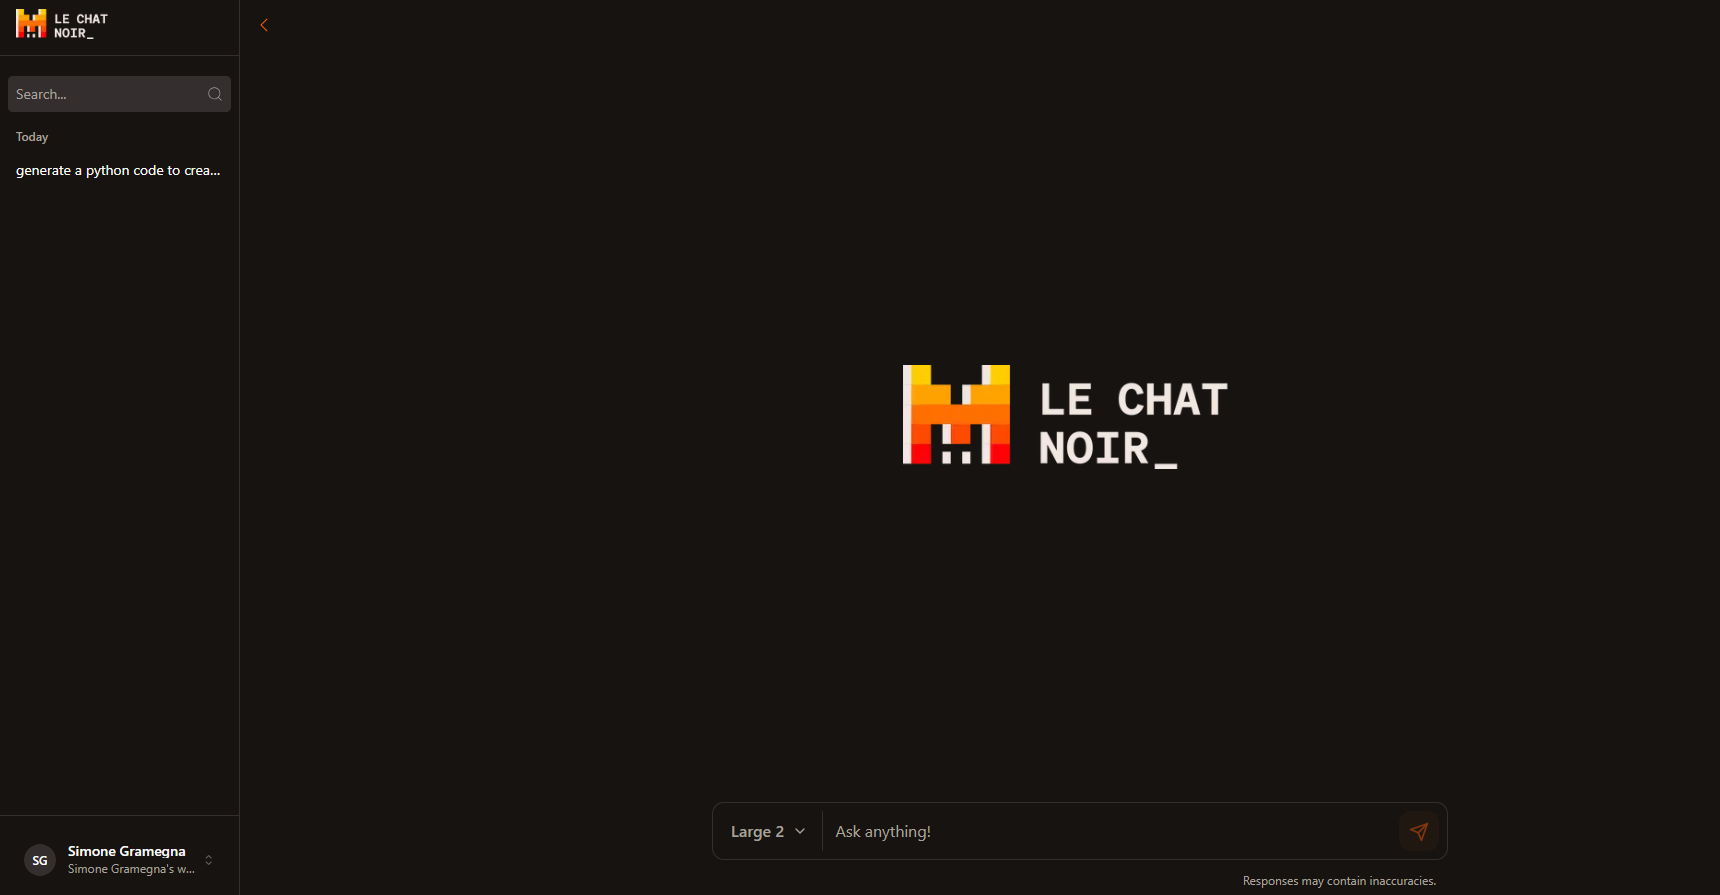
\includegraphics[width=0.9\linewidth]{Figures/fig_20.png}
    \caption{Mistral web interface}
    \label{fig_20}
\end{figure}

\subsection{Multimodal Large Language Models}
An evolution of LLMs is represented by \textit{Multimodal Large Language Models} MLLMs, which are capable of processing information in various forms: text, images, audio, video, and documents.
They are based on a modified version of the transformer architecture that is able to learn embeddings (vector representations) also of images, audio, and video. 
% Processing these embeddings through a multi-layered network generates an output in the form of text or an image\cite{wadekar2024evolution} as represented in Fig.~\ref{}.
Processing these embeddings through a multi-layered network generates outputs as text and/or media \cite{wadekar2024evolution} as represented in Fig.~\ref{fig:21}.
\begin{figure}[H]
    \centering
    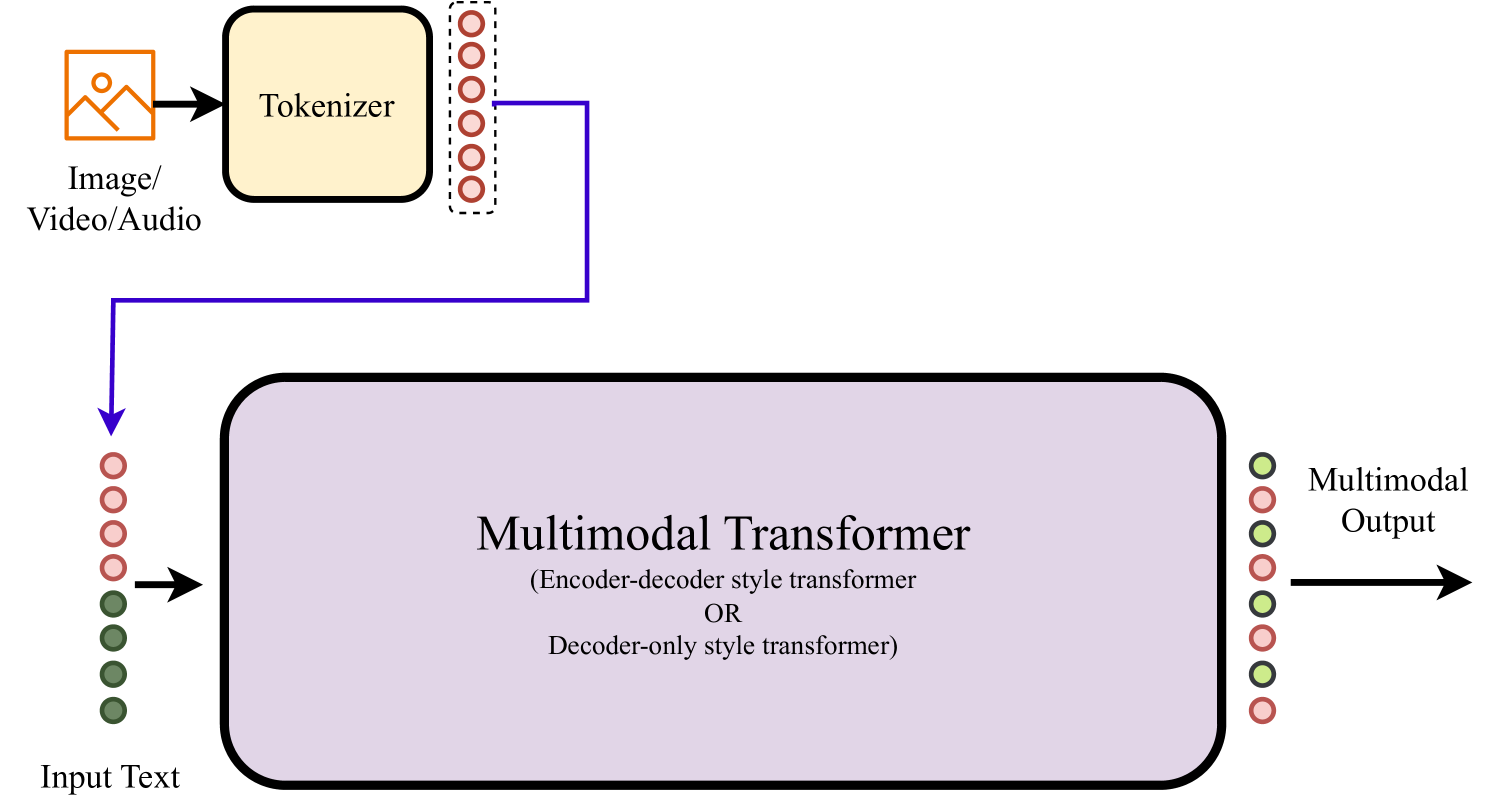
\includegraphics[width=0.9\linewidth]{Figures/fig_21.png}
    \caption{Example of multimodal transformer architecture}
    \label{fig:21}
\end{figure}

% This architecture in MLLMs is applied in order to perform two main tasks:
% \begin{enumerate}
%     \item \textbf{Image-To-Text:} assigning a textual description to an image.

%     \item \textbf{Text-To-Image:} generating an image, given a text.
% \end{enumerate}

Several MLLMs have been introduced as evolutions of classic LLMs.
We will cover the following state-of-the-art MLLMs:
\begin{itemize}
    \item \textbf{GPT-4}
    \item \textbf{Google Gemini} 
    \item \textbf{GLaMM}
\end{itemize}

GPT-4 is the latest version of the most popular LLM: GPT.
Released in March 2023, it became available to premium users of the ChatGPT platform in three distinct versions: GPT-4, GPT-4 Turbo, and GPT-4o (omni).
These versions represent an evolution of GPT-3, enhancing performance and efficiency \cite{insights_gpt4}.
The multimodal version of GPT-4, known as GPT-4o where the "o" stands for "omni," highlighting the "omniscience" that this model is capable of:
\begin{itemize}
    \item Real-time voice communication: engage in real-time voice conversations, understanding spoken input and generating natural-sounding voice responses.
    
    \item Real-time vision: process and understand vision data like images and video and their semantics. The model can generate an image starting from text and applying styles or generating descriptions of an image.
    
    \item Data and Chart Reading: read and interpret data in forms of charts and graphs.
\end{itemize}
These features make GPT-4o a versatile and powerful tool applicable in many sectors, with particular emphasis on programming and data analysis.
Details regarding the dataset, number of parameters, and training technique are not disclosed for competitive reasons.

The latest evolution of Google's LLMs is Gemini \cite{gemini_introduction}.
It has been introduced in 2023 and is the evolution of Bard: the chatbot based on PaLM, which is discussed before.
Gemini is a proprietary model and it has proven to be superior to its rival GPT-4 on various benchmarks.

\textit{Grounding LLM} (GLaMM) has been released in 2023 by Mohamed bin Zayed University of AI \cite{rasheed2024glamm}.
GLaMM is a MLLM that integrates natural language with object segmentation masks in images, combining scene-level, region-level, and pixel-level understanding.
The model uses an auto-encoder to process images and an LLM to understand natural language.
It is an open-source LLM: the source code and parameters are available on the official GitHub repository \footnote{https://github.com/mbzuai-oryx/groundingLMM}.
% \section{Prompt Engineering}
\section{Prompting}
\label{section:2_4_prompt_engineering}
% \subsection{What is prompt engineering?}
\subsection{Definition and structure}
At the core of interaction with LLMs are prompts, i.e., instructions written in natural language given as input to LLMs to generate responses \cite{llm_prompt}.
% A prompt can be written without a criterion or following specific prompting techniques that describe the structure.
% \textit{Prompt Engineering} is a novel discipline concerned with prompt writing and verification.
We can see a prompt like a mathematical function that takes in input a text and gives an output $f(x) = y$ in which $f$ is the template applied to the text of the problem.
For example, if we want to translate a phrase in English:
\begin{lstlisting}
Translate {X} in english
\end{lstlisting}
This is just a simple technique in which there is the manual creation of the template, but in literature there are more complex techniques that we are going to discuss.
In more detail, there are four main components of a prompt:
\begin{itemize}
    \item Instruction: (mandatory) a specific task or instruction you want the model to perform.
    \item Context: (optional) external information or additional context that can steer the model to better responses.
    \item Input data: (mandatory) the input or question that we are interested to find a response for.
    \item Output Indicator: (optional) the type or format of the output.
\end{itemize}

An example of output with all four components is the following:
\begin{lstlisting}
Solve the following linear equation for x and show the steps clearly. 
This is a basic algebra problem where you need to isolate x on one side of the equation.
Solve for x: 3x + 7 = 16
Provide the output in text format.
\end{lstlisting}
In this prompt the instruction is: \textit{"Solve the given linear equation for x."}, the context is: \textit{"This is a basic algebra problem where you need to isolate x on one side of the equation."}, the input data is: \textit{"Solve for x: 3x + 7 = 16"} and the output indicator is: \textit{"Provide the output in text format."}
Context and output indicator are optional components but they are useful to improve the quality of the output.




% We can see a prompt like a mathematical function that takes in input a text and gives an output $f(x) = y$ in which $f()$ is the template applied to the text of the problem, for example if we want to translate a phrase in english:
% \begin{lstlisting}
% Translate {X} in english
% \end{lstlisting}
% This is just a simple technique in which there is the manual creation of the template but there are in literature more complex techniques that we are going to discuss.

\subsection{Prompt Engineering}
% R. Richiesta modifica. Controllare la consistenza dello stile dell'espressione prompt engineering (compare come Prompt Engineering, prompt Engineering, Prompt engineering, o \textit{Prompt Engineering}. Usare sempre lo stesso.). Se ti fa comodo puoi anche definire un acronimo (PE per esempio) e usare sempre quello. Controllare la consistenza dello stile dei nomi dei prompt. Per esempio, su chain of thought il corsivo va e viene. Inoltre, a volte si chiama chain of tought, altre chain of thoughts. Verificare anche nei capitoli successivi.
% Prompt engineering techniques involve structuring a prompt in a specific way according to a particular strategy in order to obtain more accurate responses and a better understanding of the problem to be solved by the model.
\textbf{Prompt Engineering} is a novel discipline concerned with prompt writing and verification.
The first and simplest technique is the \textbf{Zero-shot prompting} in which no example is provided, and the LLM has no prior knowledge of the context, generating the output based solely on the given input prompt.
An example is the following: 
\begin{lstlisting}
Classify the text into neutral, negative or positive. 
Text: I think the vacation is okay.
Sentiment:   
\end{lstlisting}
In \textbf{Few-shot prompting}, on the other hand, the input prompt provided to the LLM includes a few examples. Examples are useful to achieve a better understanding of the context, this is not possible with zero-shot prompting, as we can see in the following example:
\begin{lstlisting}
Task: Translate the following sentences from italian to english.

Example "Oggi il tempo e' bello" output: "The weather is nice today"

input: "Mi piace leggere libri" // output: I love reading books
\end{lstlisting}

In \textbf{Chain-of-Thought (CoT) Prompting}, problem-solving is carried out step by step, breaking down a task into multiple stages to achieve more structured and accurate responses.
An example is the following:
\begin{lstlisting}
Q: Roger has 5 tennis balls. He buys 2 more cans of tennis balls. Each can has 3 tennis balls. How many tennis balls does he have now? 
A: Roger started with 5 balls. 2 cans of 3 tennis balls each is 6 tennis balls. 5 + 6 = 11. The answer is 11.  
Q: The cafeteria had 23 apples. If they used 20 to make lunch and bought 6 more, how many apples do they have?

Model output: The cafeteria had 23 apples originally. They used 20 to make lunch. So they had 23 -  20 = 3.  They bought 6 more apples, so they have 3 + 6 = 9. The answer is 9.   
\end{lstlisting}
The main issue with this technique is the manual intervention required, as the user must manually provide the reasoning that the LLM will follow.
To address this problem, a variant called \textbf{Automatic Chain-of-Thought (Auto-CoT) Prompting} was introduced.
% Instead of manually providing the reasoning chain, the prompt includes a simple phrase, "Let's think step-by-step," to automatically generate multiple reasoning chains.\\
Instead of manually providing the reasoning chain, the prompt includes the simple phrase, \textit{``Let's think step-by-step``} 
% R. verificare
for eliciting the model to engage in a CoT without adding examples of step-by-step problem solving in the prompt.
% for automatically generating multiple examples that are useful to solve the input problem, encouraging the model to "think step-by-step".
Both CoT and Auto-CoT follow a single reasoning path, but we can generate multiple reasoning paths and choose the best answer; this is the basis of the \textbf{Self-consistency prompting} \cite{wang2022self}.
Techniques involving multiple prompts are useful in order to decide the best reasoning strategy but we can also decide not to use any complex reasoning, but a more simple strategy that can involve the ensembling, the augmentation, the composition or the decomposition of a single prompt \cite{liu2023pre}.
In \textbf{prompt ensembling}, different prompts are combined on the same input in order to get a response. For instance:
\begin{lstlisting}
PR1: China's capital is [X]
PR2: [X] is capital of China
PR3: The capital of China is [X]
\end{lstlisting}

% R. Spiegazione modifica. evitare "ecc"
% To choose the response, we can apply several strategies, including majority voting, weighted voting ecc..
To choose the response, we can apply several strategies, including majority voting and weighted voting.
In \textbf{prompt composition} there is a composition of two or more subprompts in order to get the final prompt.
In contrast, in \textbf{prompt decomposition} one main prompt is decomposed in two or more smaller subprompts.
% R. Nota. Nei commenti precedenti ti ho suggerito di parlare di questo problema nella sezione su LLM. Se segui i commenti qui puoi evitare di definire di nuovo le hallucinations.
In LLMs, there is a significant issue that leads to incorrect responses, known as the problem of hallucinations.
We refer to hallucination, in the context of LLMs, when there is the generation of texts or responses that are grammatically and syntactically correct but deviate from the given inputs or do not align with factual accuracy \cite{ye2023cognitive}.
Prompt engineering techniques can help reduce this phenomenon, the main technique is \textbf{Retrieval Augmented Generation} (RAG).
In this approach, starting from an input, a knowledge base of sources (web pages, articles, etc.) is created, and the text from these sources is incorporated into the subsequent input, providing context and generating more accurate and reliable responses.
% R. Richiesta modifica. Cosa sono le task-solving trajectories? Queste cose human written sono inserite come esempi nel prompt?
The improvement in performance and accuracy of the responses obtained from the LLM can also be achieved by incorporating the user's emotions into the prompt, known as \textbf{Emotion Prompting}.
Incorporating emotions can be useful in tasks such as sentiment analysis of a sentence, but this is not the case for code generation, for which various prompt engineering techniques have been introduced.
% R. Richiesta modifica. Siamo tornati ai prompt che fanno "ragionamento"?? Spostare questa parte dopo graph-of-thought
An evolution of the previously described Chain-of-Thoughts is \textbf{Program of Thoughts (PoT) Prompting} \cite{chen2022program}, where the large language model is given a prompt containing intermediate steps that include mathematical expressions or source code, as we can see in the following figure:
\begin{figure}[H]
    \centering
    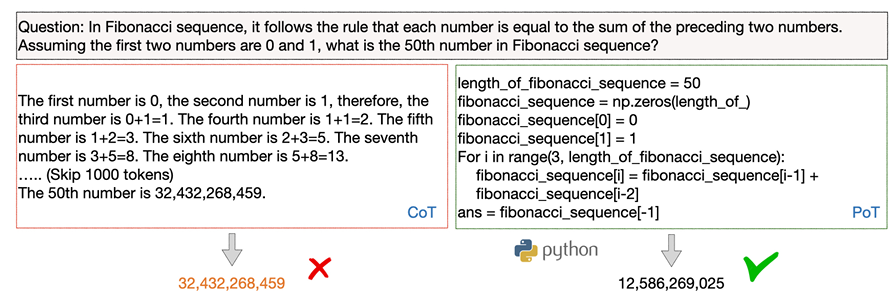
\includegraphics[width=0.7\linewidth]{Figures/fig_8.png}
    \caption{Program of Thoughts (PoT) Prompting}
    \label{fig:enter-label}
\end{figure}
Another approach is the \textbf{Scratchpad Prompting} in which an arbitrary sequence of intermediate tokens is generated before the final answer is provided. 
The sequence is given in a tag called "scratch" \cite{scratch,nye2021show} in which the user writes intermediate steps useful to the LLM as shown below, were it is requested to solve a simple mathematical problem:
The problem is: A store sells apples for 3 euros each. If I buy 5 apples and get a 10\% discount, how much do I pay in total?
\begin{lstlisting}
<scratch>
Perform the following calculations step by step. Write your notes in the format "Scratchpad:" for each step.

Problem: A store sells apples for 3 euros each. If I buy 5 apples and get a 10% discount, how much do I pay in total?

Scratchpad:
1. The unit price of an apple is 3 euros.
2. The number of apples purchased is 5.
3. The total cost without discount is: 3 * 5 = 15 euros.
4. The 10% discount is: 15 * 0.10 = 1.5 euros.
5. The final price after the discount is: 15 - 1.5 = 13.5 euros.
Final result: 13.5 euros.
</scratch>
\end{lstlisting}
In the example above, we begin the sequence with $<scratch>$ and we define the different steps that the model has to follow in order to solve the problem. The sequence ends with $</scratch>$.

% R. Richiesta modifica. Spiegare la sintassi usato per lo scratch in questo esempio, non è semplicissima da comprendere
%% SG: modificato esempio. Non si capiva molto

The \textbf{Rephrase and Respond (RaR) Prompting}\cite{deng2023rephrase} technique automatically allows for the correction and improvement of the LLM's response through the prompt:
\begin{lstlisting}
"{question}" Rephrase and expand the question, and respond.
\end{lstlisting}
This approach has four main advantages:
\begin{enumerate}
    \item It lets the LLM self-improve the prompts while maintaining the context of the original query.

    \item It allows better aligning the human’s intended query with LLM’s preferred style of question.

    \item It expands the LLM’s thought process and adding a step that will not naturally appear when using CoT.

    \item It provides an approach for humans to interpret how LLMs understand the questions.
\end{enumerate}
% R. Richiesta modifica. Correggere il riferimento alla figura. fatto
Another technique to obtain more accurate and comprehensive responses is the \textbf{Take a Step Back Prompting}\cite{zheng2023take}, which consists of two steps. The first step involves inputting a specific question, and subsequently (step-back) inputting a more abstract, high-level question related to the task, as shown in the following figure:
\begin{figure}[H]
    \centering
    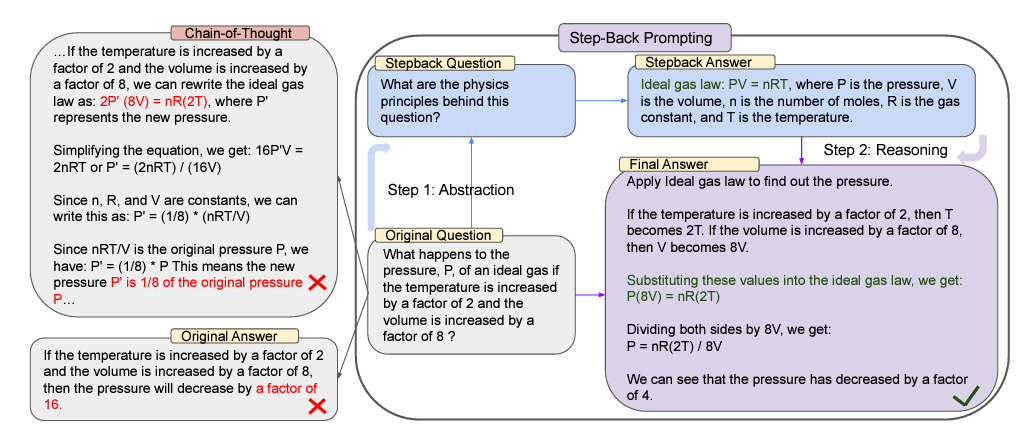
\includegraphics[width=0.9\linewidth]{Figures/fig_9.png}
    \caption{Take a Step Back Prompting}
    \label{fig:9}
\end{figure}

\subsection{Prompt engineering in multimodal LLMs}
State-of-the-art prompt engineering techniques aim, when given as input to a LLM, to generate text.
MLLMs allow for incorporating media such as image into prompts.
Main tasks involving MLLMs are:
\begin{itemize}
    \item Image generation
    \item Image classification
    \item Image editing
\end{itemize}

A preliminary approach to image classification is the use of zero-shot prompting and few-shot prompting \cite{chen2023unleashing}.
In zero-shot prompting for image generation, no input examples are provided, but only the instruction to be executed, for example:
\begin{lstlisting}
Classify the follwing image: [image.png]
\end{lstlisting}
In few-shot prompting, examples are provided to the model, for instance:
\begin{lstlisting}
Given: [image1.png], [image2.png], [image3.png], classify the following image: [image.png]
\end{lstlisting}
% R. Spiegazione modifica. Frase spezzata e semplificata. Trovo spesso più frasi che aggiungono tante informazioni divise solo con la virgola. Usare le congiunzioni.
% Zero-shot prompting and few-shot prompting can be also used in image generation, this task is more complex and it can be useful to incorporate user feedback that helps improve the generated image. ok
Zero-shot prompting and few-shot prompting can be also used in image generation.
However, this task is more complex and it can benefit from user feedback.
An example is drawing a stick figure using letters of the alphabet \cite{proptingguide_image}, where the process starts from an initial prompt, such as:
\begin{lstlisting}
Produce TikZ code that draws a person composed from letters in the alphabet. The arms and torso can be the letter Y, the face can be the letter O (add some facial features) and the legs can be the legs of the letter H. Feel free to add other features.    
\end{lstlisting}
The generated image is refined by adding details: 
\begin{lstlisting}
- The torso is a bit too long, the arms are too short 
  and it looks like the right arm is carrying the face instead of the face being right above the torso. Could you correct this please? 

- Please add a shirt and pants.
\end{lstlisting}
As we can see in the following example, where the latest version of ChatGPT, GPT4, has been applied:
\begin{figure}[H]
    \centering
    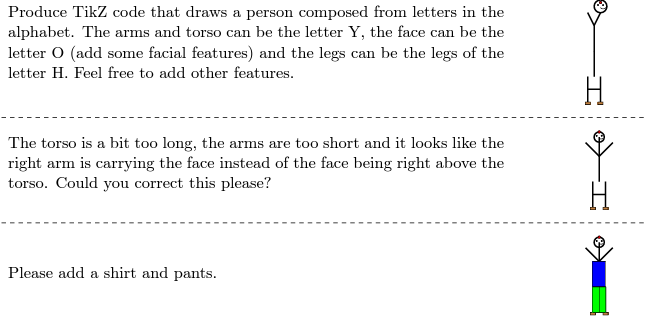
\includegraphics[width=0.8\linewidth]{Figures/fig_10.png}
    \caption{Drawing using GPT4}
    \label{fig:10}
\end{figure}
In image generation the characteristics of an image can be specified not only using user feedback but also using \textbf{style modifiers}.
They are descriptors that consistently produce certain styles, for example: "tinted red", "made of glass", and combining those together they produce a more specific style \cite{lp_style}.
% R. Spiegazione modifica. un po di punteggiatura, altrimenti non si capisce nulla. ok
For example, we want to generate, using DALL-E, a picture of a pyramid.
% R. Richiesta modifica. Referenziare correttamente la figura. fatto
The first picture is generated without using any modifier:
\begin{figure}[H]
    \centering
    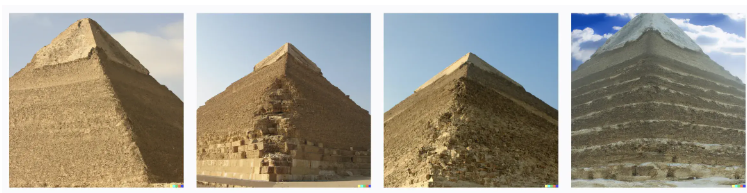
\includegraphics[width=0.9\linewidth]{Figures/fig_11.png}
    \caption{Pyramid picture with no modifiers}
    \label{fig:11}
\end{figure}
The second picture is generated using the prompt with three modifiers: \textit{A pyramid made of glass, rendered in Unity and tinted red} getting the following result:
% R. Richiesta modifica. Referenziare correttamente la figura. fatto
\begin{figure}[H]
    \centering
    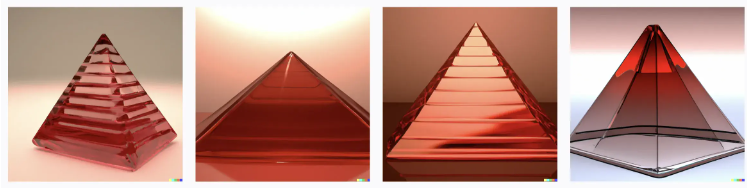
\includegraphics[width=0.9\linewidth]{Figures/fig_12.png}
    \caption{Pyramid picture with modifiers}
    \label{fig:12}
\end{figure}
In the prompt, in order to improve quality, we can add generic adjectives like: \textit{"amazing"}, \textit{"good"}, \textit{"beautiful"} that are called \textbf{quality boosters} \cite{oppenlaender2023taxonomy}.
The Latin motto \textit{"repetita iuvant"} that means that repeating words is useful can be applied in a certain sense in a prompt for image generation, the \textbf{repetition technique} gives more importance to some adjective instead of another it is possible to repeat more times the word, giving emphasis to it.
% R. Richiesta modifica. brutto "if we want". sembra una frase parlata.
For example, the generation of an image of a waterfall, but we want to emphasise the beauty of the picture we can use this following prompt:
\begin{lstlisting}
A very very very very very beautiful painting of a mountain next to a waterfall
\end{lstlisting}
In this case the word "very" is repeated five times in order to give more importance to the adjective beautiful.
% R. Spiegazione modifica. Senza i connettivi non si capisce nulla.
Since repeating terms in a prompt can be weird and inaccurate, it is possible to use \textbf{weighted terms technique}\cite{weighted_terms}, in which a term has a numerical value (positive or negative) that corresponds to the weight, i.e., the importance of that term.
% R. Richiesta modifica. Brutto "we want". Sembra una frase parlata. ok
For example, the generation of a picture of a mountain without trees, we use this prompt:
\begin{lstlisting}
mountain | tree:-10.
\end{lstlisting}
% R. Richiesta modifica. Referenziare correttamente la figura.
in which the tree has negative weight and it doesn't have importance getting this result, as we can see in the figure \ref{fig:15}:
\begin{figure}[H]
    \centering
    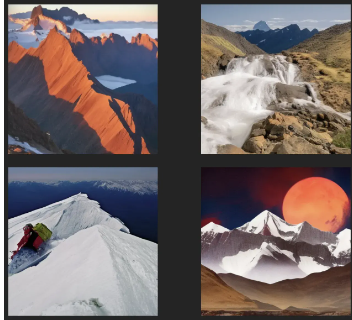
\includegraphics[width=0.5\linewidth]{Figures/fig_15.png}
    \caption{Weighted terms image}
    \label{fig:15}
\end{figure}

% R. Richiesta modifica. Negative prompts ripetuto tre volte a breve distanza.
Another approach in image generation is negative prompting, those allow users to exclude unwanted features and enhance the quality output.
Negative prompts are complementary to  positive prompts which describe what the user wants, including the main subject and how it should look \cite{medium_negative}.
For example, we want to generate using a diffusion model a portrait of a man without mustache, so the prompt is:
\begin{lstlisting}
- Positive prompt: Portrait photo of a man.
- Negative prompt: Mustache
\end{lstlisting}
Negative prompts can be applied on any image feature like: colors, lighting problems, unwanted elements, image quality and style.
% R. spiegazione modifica. usato l'acronimo e rimosso il titolo dello studio
% Multimodal large language models can be used not only to generate photorealistic images, but also artistic images following the style of a particular artist or artistic movement, as discussed in the paper \textit{Design Guidelines for Prompt Engineering Text-to-Image Generative Models} \cite{liu2022design}.
% R. Spiegazione modifica. Spezzata frase ingarbugliata. Aggiunto spazio prima del riferimento.
% The \textbf{Multimodal Chain-of-Thought} prompting technique\cite{zhang2023multimodal} is a variation of the Chain-of-Thought technique (CoT), this technique in Multi-CoT is enhanced by incorporating in the prompt text and visual inputs.
The \textbf{Multimodal Chain-of-Thought} prompting technique \cite{zhang2023multimodal} is a variation of the Chain-of-Thought technique (CoT).
This technique in Multi-CoT is enhanced by incorporating in the prompt text and visual inputs.
The technique consists in two stages:
\begin{enumerate}
    \item Rationale generation: the model processes the multimodal inputs in order to generate an intermediate reasoning chain (rationale). The rationale explains the logical steps required to arrive at the final answer, using both textual and visual content as context.

    \item Answer inference: the generated rationale is combined with the original input and used by the model to infer the final answer.
\end{enumerate}
% R. Richiesta modifica. Referenziare correttamente la figura e iniziare con la maiuscola perchè hai chiuso le frasi col punto nell'elenco numerato. ok
as we can see in the figure \ref{fig:16} below:
\begin{figure}[H]
    \centering
    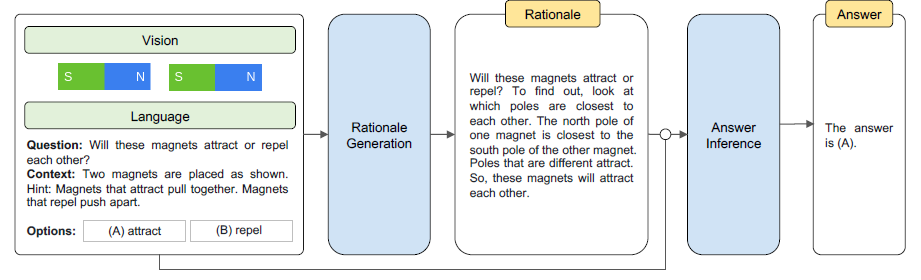
\includegraphics[width=0.9\linewidth]{Figures/fig_16.png}
    \caption{Multimodal Chain-of-Thought}
    \label{fig:16}
\end{figure}
% R. Spiegazione modifica. Rimosso perchè dettaglio.
% The technique has been tested on T5, UnifiedQA and FLAN-Alpaca and it has a good accuracy averaging around 85\%.
Similar to the multimodal chain-of-thought, the \textbf{Chain of Images (CoI)} prompting technique \cite{meng2023chain} generates a series of images as intermediate representations in order to solve problems starting from a textual prompt.
% R. Richiesta modifica. Non è stato detto prima cosa è SyMLLM 
% SG: tolto
